\documentclass[12pt]{report} 
\usepackage[utf8]{inputenc}
\usepackage{geometry}
\geometry{letterpaper}
\usepackage{graphicx} 
\usepackage{parskip}
\usepackage{booktabs}
\usepackage{array} 
\usepackage{paralist} 
\usepackage{verbatim}
\usepackage{subfig}
\usepackage{fancyhdr}
\usepackage{sectsty}

\pagestyle{fancy}
\renewcommand{\headrulewidth}{0pt} 
\lhead{}\chead{}\rhead{}
\lfoot{}\cfoot{\thepage}\rfoot{}


%%% ToC (table of contents) APPEARANCE
\usepackage[nottoc,notlof,notlot]{tocbibind} 
\usepackage[titles,subfigure]{tocloft}
\renewcommand{\cftsecfont}{\rmfamily\mdseries\upshape}
\renewcommand{\cftsecpagefont}{\rmfamily\mdseries\upshape} %

\usepackage{amsmath}
\usepackage{amssymb}
\usepackage{empheq}
\usepackage{xcolor}

\usepackage{tikz}

%\usepackage{pgfplots}
%\pgfplotsset{width=10cm,compat=1.9}

% We will externalize the figures
%\usepgfplotslibrary{external}
%\tikzexternalize

\renewcommand{\L}[1]{\mathcal{L}\{#1\}}
\newcommand{\ans}[1]{\boxed{\text{#1}}}
\renewcommand{\hat}[1]{\widehat{#1}}
\newcommand{\F}[1]{\mathcal{F}(#1)}
\renewcommand{\P}{\mathbb{P}}
\newcommand{\R}{\mathbb{R}}
\newcommand{\qed}{\quad \blacksquare}
\newcommand{\brak}[1]{\langle #1 \rangle}
\newcommand{\Z}{\mathbb{Z}}

\title{Math 1530: Abstract Algebra}
\author{Milan Capoor}
\date{Fall 2023}

\begin{document}
\maketitle
\chapter*{Groups}
\section*{Lecture 1: Sept 7}
Richard Schwartz
\begin{itemize}
    \item richard.evan.schwartz@gmail.com
\end{itemize}

\subsection*{The Cube}
Let $G$ be the set of symmetries of the cube. Given $a,\;b \in G$, $a \star b$ is the concatenation of $a$ and $b$

Notice:
\begin{itemize}
    \item $(a \star b) \star c = a \star (b \star c)$ (associative)
    \item $\exists e \text{ such that } e\star a = a \star e = a \; \forall a \in G$ (identity)
    \item $\forall a \in G \; \exists \, b \text{ such that } a\star b = e$ (inverse)
\end{itemize}

\textbf{A group is anything that satisfies these axioms}

\textbf{Examples of groups:}
\begin{itemize}
    \item Permutations of the Rubik's Cube
    \item the integers
    \item $\Z // n := \{0, \, ..., n -1\}$ (``Z mod n'' where $Z // 12$ would work like a clock)
\end{itemize}

Structures heuristically:
\begin{itemize}
    \item A group is a set with addition/concatenation
    \item A ring is a group plus multiplication
    \item A field is a ring plus division and commutativity
\end{itemize}

\section*{Lecture 2: Sept 12}
\subsection*{Groups}
\textbf{Group:} a group is a set $G$ with an operation $\star: G \times G \to G$ such that 
\begin{enumerate}
    \item $\star$ is always defined 
    \item $a \star (b \star c) = (a \star b) \star c \quad \forall a, b, c \in G$ (Associativity)
    \item $\exists e \in G, \text{ such that } e \star a = a \star e = a \quad \forall a \in G$ (Identity)
    \item $\forall a \in G, \; \exists b \in G, \text{ such that } a \star b = b \star a = e$ (Inverses)
\end{enumerate}

\textbf{Lemma 1:} In a group, $e$ is unique.

\emph{Proof:} 
\begin{enumerate}
    \item Suppose $e$ and $e'$ are both identity elements of the group $G$.
    \item Consider $e \star e'$
    \item Since $e$ is an identity, $e \star e' = e'$
    \item But since $e'$ is an identity, $e \star e' = e$
    \item Therefore, $e' = e \qed$
\end{enumerate} 

\textbf{Lemma 2:} Suppose $a \star c_1 = a \star c_2$. Then, $c_1 = c_2$. 

\emph{Proof:}
\begin{enumerate}
    \item Let $b$ be an inverse of $a$
    \item Since $a \star c_1 = a \star c_2$, 
    \[b\star (a \star c_1) = b \star (a \star c_2)\]
    \item Then by associativity, 
    \[(b \star a) \star c_1 = (b \star a) \star c_2\]
    \item By the definition of inverses, $(b \star a) = e$ so
    \[e \star c_1 = e \star c_2\]
    \item And by identity, 
    \[c_1 = c_2 \qed\]
\end{enumerate}

\textbf{Lemma 3:} Inverses are unique ($\forall a \in G \quad \exists ! b \in G \text{ such that } a \star b = b \star a = e$)

\emph{Proof:}
\begin{enumerate}
    \item Suppose $b_1$ and $b_2$ are both inverses of $a$
    \item Then, 
    \[a \star b_1 = e = a \star b_2\]
    \item By lemma 2, $b_1 = b_2 \qed$
\end{enumerate}

\subsection*{Examples of Groups}
\textbf{Permutation groups:} The set of all bijective maps from $S \to S$ (the maps that hit every element in the codomain exactly once)

\textbf{Surjective:} onto; each element of the codomain is mapped to by at least one element of the domain.

\textbf{Injective:} one-to-one; each element of the codomain is mapped to by at most one element of the domain
  
Permutation groups can be represented by arrow diagrams, tables, pairs, and cycles. For example, 
\begin{center}
    \begin{tabular*}{0.78 in}{|c|c|}
        \hline
        $S$ & $g(S)$\\
        \hline
        1 & 5\\
        2 & 8\\
        3 & 3\\
        4 & 6\\
        5 & 1\\
        6 & 9\\
        7 & 7\\
        8 & 4\\
        9 & 2\\
        \hline
    \end{tabular*}
\end{center}

is the same as 
\[\begin{pmatrix}
    1 & 2 & 3 & 4 & 5 & 6 & 7 & 8 & 9\\
    5 & 8 & 3 & 6 & 1 & 9 & 7 & 4 & 2
\end{pmatrix}\]
which is also equivalent to 

\usetikzlibrary{chains}
\begin{center}
    \begin{tikzpicture}[start chain=circle placed {at=(\tikzchaincount*40:4)}]
        \foreach \i in {1,...,9}
          \node [on chain] {\i};
      
        \draw[bend left,->]  (circle-1) to node [auto] {} (circle-5);
        \draw[->] (circle-2) -- (circle-8);
        \draw[->] (circle-4) -- (circle-6);
        \draw[bend left,->]  (circle-5) to node [auto] {} (circle-1);
        \draw[->] (circle-6) -- (circle-9);
        \draw[->] (circle-8) -- (circle-4);
        \draw[->] (circle-9) -- (circle-2);
        \draw[->] (circle-3.north) arc[start angle=0, end angle=270, x radius=0.3cm, y radius=0.3cm];
        \draw[->] (circle-7.south) arc[start angle=0, end angle=-270, x radius=0.3cm, y radius=0.3cm];

    \end{tikzpicture}
\end{center}

which can be notated
\[(3)(7)(15)(28469)\]

\subsection*{Homomorphisms}
\textbf{Homomorphism:} a map between groups $G_1$ and $G_2$, $\phi: G_1 \to G_2$ such that $\phi(a \star_1 b) = \phi(a) \star_2 \phi(b)$

\textbf{Example:} $G_1$ is rotations of a pentagon and $G_2 = \Z/5$

\textbf{Isomorphism:} a bijective homomorphism

\section*{Lecture 3: Sept 14}
\textbf{Recall:} a homomorphism is a map $\phi : G_1 \to G_2:$
\[\phi(a \star_1 b) = \phi(a) \star_2 \phi(b)\] 

\textbf{Lemma:} Let $\phi$ be a homomorphism from $G_1 \to G_2$. Then $\phi(g^{-1}) = (\phi(g))^{-1} \quad \forall g \in G_1$

\emph{Proof:} 

\begin{align*}
    \phi(e) &= e\\
    g\cdot g^{-1} &= e\\
    e = \phi(g\cdot g^{-1}) &= \phi(g) \cdot \phi(g^{-1}) \quad \; \text{ by homomorphism}\\
    e &= \phi(g) \cdot (\phi(g))^{-1} \quad \text{ by definition of inverse}\\
    \phi(g^{-1}) &= (\phi(g))^{-1} \qquad \quad \text{ by cancellation} \qed
\end{align*}

\subsection*{Subgroups}
\textbf{Kernel:} Let $\phi : G_1 \to G_2$ be a homomorphism. Then 
\[\ker(\phi) := \phi^{-1}(e) = \{a \in G_1 | \phi(a) = e\}\]

\textbf{Lemma:} $\ker(\phi)$ is a subgroup of $G_1$

\emph{Proof:}
\begin{enumerate}
    \item Suppose $a, b \in \ker(\phi)$
    \[\phi(ab) = \phi(a)\phi(b) = ee = e \quad \checkmark\]
    
    \item Suppose $a^{-1} \in \ker(\phi)$
    \[\phi(a^{-1}) = [\phi(a)]^{-1} = e^{-1} = e \quad \checkmark\]
\end{enumerate}
Therefore $\ker(\phi)$ is closed under multiplication and inverses, so it is a subgroup. $\qed$

\textbf{Theorem:} $\phi$ is one-to-one (injective) if and only if $\ker(\phi) = \{e\}$

\emph{Proof:}

$\phi(e) = e$ so $\phi(g) \neq e$ if $g \neq e$. Therefore, $\ker(\phi)$ must be $\{e\}$

Now for the other direction, suppose $\phi(x) = z$ and $\phi(y) = z$. We then know $\phi(y^{-1}) = z^{-1}$, so 
\[\phi(y^{-1})\phi(x) = z^{-1} \phi(x) = z^{-1}z = e\]
Because $\phi$ is a homomorphism, 
\[\phi(y^{-1}) \phi(x) = \phi(y^{-1}x)\]
so 
\[y^{-1}x \in \ker(\phi) \implies y^{-1}x = e \implies x = y \qed\]

\subsection*{More generally}
Let $\phi: G_1 \to G_2$ be a homomorphism and $H_2$ a subgroup of $G_2$, 
\[\phi^{-1}(H_2) = \{a\in G_1 | \phi(a) \in H_2\}\]

\emph{Lemma:} $\phi^{-1}(H_2)$ is a subgroup of $G_1$

\textbf{Proof:} 
\begin{enumerate}
    \item Identity: $\phi(e) = e \quad e \in \phi^{-1}(H_2)$
    \item Multiplication closure: $a, b \in \phi^{-1}(H_2)$, 
    \[\phi(ab) = \phi(a)\phi(b) \in H_2 \quad \text{ $H_2$ is closed under products}\]
    so $ab \in \phi^{-1}(H_2)$

    \item Inverse closure: $a \in \phi^{-1}(H_2)$ 
    \[\phi(a^{-1}) = [\phi(a)]^{-1} \in H_2 \quad \text{ $H_2$ is closed under inverses}\]
    so $a^{-1} \in \phi^{-1}(H_2)$
\end{enumerate}

\subsection*{Interlude: Cube notation}
Let 
\begin{center}
    $ a = $ 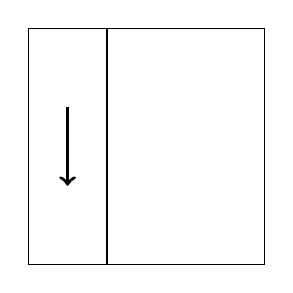
\begin{tikzpicture}[baseline={([yshift=-.5ex]current bounding box.center)}]
        \draw (0, 0) rectangle (1, 3);
        \draw (1, 0) rectangle (3, 3);
        \draw[very thick, ->] (0.5, 2) -- (0.5, 1);
    \end{tikzpicture}
\end{center}

This means that we turn the left face down.

Notice that after four turns, we have returned to the beginning, so 
\[aaaa = a^4 = e\]
which creates a (cyclic) subgroup of the cube,
\[H = \{e, a, a^2, a^3\}\]

\textbf{Notation:} Given $G$ and $a \in G$, 
\[\brak{a} = \{a^k, \; k \in \Z\}\]'

\textbf{Why are the symmetries of the cube not a cyclic group?}

There is no generator of order 24. 

OR cyclic groups are abelian. 
\[a^m a^n = a^{m + n} = a^{n + m} = a^n a^m\]

\section*{Lecture 4: Sept 19}
\subsection*{Review}
\textbf{Recall:} A homomorphism is a map $\phi: G_1 \to G_2$ such that 
\begin{align*}
    \phi(ab) = \phi(a)\phi(b)\\
    \phi(e_1) = e_2\\
    \phi(g^{-1}) = (\phi(g))^{-1} 
\end{align*}

\textbf{To confirm $H$ is a subgroup:} check that it is closed under multiplication and inverses. You do not need to show associativity because that is always true. 

\textbf{Generators:}
Let $G = \{a, a^2, a^3, \dots\}$ If $a^m = a^n \quad m < n$ then 
\begin{align*}
    a^{n - m} = e\\
    a^k = e \qquad (k=n - m)\\
    (a^{k-1}) a = e\\
    a^{k-1} = a^{-1}
\end{align*}

\textbf{Are Abelian Groups always cyclic?}
\emph{Answer:} No. Counterexample:
\[\Z/2 \times \Z/2 = \{(a, b) | \; a, b \in \Z/2\} = \{(0,0), (0, 1), (1, 0), (1,1)\}\]
has no generator. 

\subsection*{(Left) Cosets}
\textbf{Definition:} Given a group $G$ and a subgroup $H \subset G$, a \emph{left coset} is a set of the form 
\[aH = \{ah\; | \; h \in H\}\]
where $a \in G$

If $a \in H$, then $aH = H$. 
(Notice that for all $s \in H$, $a(a^{-1}s) = s$ and $a^{-1}s \in H$)

This all leads to the observation that \emph{every set of cosets contains the subgroup.}

\textbf{Lemma:} $H$ and $aH$ are the same size (there is a bijection from $H$ to $aH$)

\emph{Proof:} Define $\psi(h) = ah$. By definition, $aH = \psi(H)$ so $\psi$ is onto. Now suppose $\psi(h_1) = \psi(h_2)$. Then $ah_1 = ah_2$ which by cancellation shows $h_1 = h_2$. Thus, $\psi$ is one-to-one. Therefore, $\psi: H \to aH$ is a bijection. $\qed$

\textbf{Lemma:} If $aH \cap bH \neq \emptyset$, then $aH = bH$.

\emph{Proof:} Pick an element in common: $ah_1 = bh_2$. Then 
\[a = bh_2h_1^{-1}\]
so for any $h\in H$,
\[ah = b(h_2 h_1^{-1}h) \in bH\]
Since this is true for all $h \in H$, we know that $aH \subset bH$. 

Interchanging $a$ and $b$ shows that $aH = bH. \qed$

\subsection*{Lagrange's Theorem}
\textbf{Theorem:} If $G$ is a finite group and $H \subset G$ is a subgroup, then $o(H) |\; o(G)$ (The order of $H$ divides the order of $H$.) 

\emph{Proof:} Look at all the cosets and denote the number of cosets $n$. We know
\begin{enumerate}
    \item For any $g\in G$, $g=ge \in gH$ (every element is in a coset)
    \item All cosets have $o(H)$ elements (from the bijection)
    \item The cosets are mutually exclusive
\end{enumerate}
So $o(G) = n \cdot o(H) \qed$

\textbf{Corollary:} If $g \in G$ and $G$ is a finite group, then $o(g) | o(G)$

\emph{Proof:} Let $H = \brak{g}$. Then $o(H) = o(g)$. Since $o(H) |\; o(G)$ (by Lagrange's), $o(g) |\; o(G). \qed$

\section*{Lecture 5: Sept 21}
\subsection*{Recall}
\textbf{Lagrange's Theorem:} $H \subset G \implies o(H) |\; o(G)$

\textbf{Corollary of Lagrange's Theorem:} if $g \in G$, $o(g) |\; o(G)$

\subsection*{Equivalence Relations}
\textbf{Relation:} a relation on a set $S$ is a subset $R \in S \times S$
\[x \; R \; y \implies (x, y) \in R\]

\textbf{Equivalence Relation:} a relation $x \sim y$ such that $(x, y) \in R$ and 
\begin{enumerate}
    \item $x \sim x \quad \forall x \in S$
    \item $x \sim y \implies y \sim x \quad \forall x, y \in S$
    \item $x \sim y, \; y \sim z \implies x \sim z \quad \forall x, y, z \in S$
\end{enumerate}

\textbf{Example:} $H \subset G$ with $a \sim  b$ if $a^{-1} b \in H$ 

\begin{align}
    a \sim a &\implies a^{-1}a \in H \implies e \in H \checkmark\\
    a \sim b &\implies a^{-1}b \in H \implies (a^{-1}b)^{-1} = (b^{-1}a)^{-1} \implies b \sim a \checkmark\\
    a\sim b, \; b \sim c &\implies a^{-1}b, b^{-1}c \in H \implies a^{-1}x \in H \implies a \sim c \checkmark
\end{align}

\textbf{Remark:} if two equivalence classes overlap, they are the same 
\emph{Proof:} an equivalence class is a coset 

\textbf{Example:}
\begin{align*}
    a^{-1}b \in H\\
    a^{-1}b = h \in H\\
    b = ab \in aH
\end{align*}

\subsection*{The group $(\Z/n)^*$}
\textbf{Relatively Prime:} $a, b \in \Z$ are \emph{relatively prime} if $\gcd(a, b) = 1$

\textbf{Lemma:} if $a, b$ are relatively prime then $\exists s, t$ such that 
\[as + bt =1\]

\emph{Proof:}

$\impliedby$ suppose $as + bt = 1$ and $d$ divides $a, b$. Clearly, $d | as$ and $d | bt$ for $s, t\in \Z$. By distribution, 
\[d| as + bt = 1 \implies d | 1 \implies d = 1\]

$\implies$ Let $a, b$ be the smallest pair with $a < b$. Consider $a, b - a$. If $a$ and $b-a$ are relatively prime, then 
\[s'a + t'(b- a) = 1 = (\underbrace{s'- t'}_s) a + \underbrace{t'}_tb = 1\]

To show that $a$ and $b- a$ are relatively prime, we suppose $d | a$ and $d | b-a$ so $d | a + (b-a)$ so $d |b$. Using the first part of the proof, we know have $as + bt =1$ for the smallest pair we did not know we could write that way. Thus it is true for all numbers.

\textbf{Definition:} $(\Z/n)^*$ is the subset of $\{1, \dots, N\}$ which is relatively prime to $N$ together with group law multiplication and reduction.
\[(\Z/15)^* = \{1, 2, 4, 7, 8, 11, 13, 13, 14\}\]

\emph{Example:} $7\cdot 8 = 56 - (15*3) = 11 \in (\Z/15)^* $

We now consider $a, b \in (\Z/15)^*$ 
\[\begin{cases}
    1 = s_1 a + t_1 N\\
    1 = s_1 b + t_2 N\\
    1 = s_1 s_av + \dots N
\end{cases} \implies ab \in (\Z/15)^*\] 
(so identity)

\textbf{Inverses in $(\Z/N)^*$:}
\begin{align*}
    a \in (\Z/15)^*\\
    as + tN = 1\\
    s = a^{-1}\\
    aa^{-1} + tN = 1
\end{align*}
(so inverses mod multiples are in the group)

\textbf{Order of $(\Z/15)^*$:} 
\[\phi(n) := o(\Z/15)^*\]

We have $\phi(15) = 8$, $\phi(17) = 16$, etc.

In general, if $p$ is prime then $\phi(p) = p -1$ and if $p, q$ are prime then $\phi(pq) = (p - 1)(q - 1)$

\[\boxed{\frac{\phi(N)}{N} = \prod_{p | n} 1 - \frac{1}{p}}\]
\emph{Example:} $N=12, \quad (\Z/12)^* = \{1, 5, 7, 11\}$
\[\frac{\phi(12)}{12} = (1 - \frac{1}{2})(1 - \frac{1}{3}) = \frac{1}{3} \implies \phi(12) = 4\]

\subsection*{RSA Cryptography}
\textbf{Corollary of Lagrange's Theorem:} If $a$ is relatively prime to $N$ then 
\[a^{\phi(N)} \equiv 1 \mod n\]

\textbf{The Algorithm:}
\begin{enumerate}
    \item Pick two very large primes $p, q$ (choose very big numbers and check if they are prime)
    \item publish the value of $N = pq$ 
    \item Keep secret the number $\phi(N) = (p-1)(q-1)$
    \item Choose a public $E$ relatively prime to $\phi(N)$ ($DE + k\phi(N) = 1$) where $D$ is your private ``decoder''
\end{enumerate}

\chapter*{Rings}
\section*{Lecture 6: Sept 26}
\textbf{Ring:} a set $R$ with two operations (usually $+$, \; $\cdot$) such that:
\begin{enumerate}
    \item $(R, +)$ is an abelian group 
    \item $(R, \cdot)$ is a ``group'' which may or may not have inverses (the operation is always defined, it is associative, and there is an identity) 
    \item 
    \[\forall a, b, c \in R : \quad \begin{cases}
        a \cdot (b + c) = a\cdot b + a \cdot c\\
        (b + c) \cdot a = b\cdot a + c\cdot a
    \end{cases}\]
\end{enumerate}

We usually call $1$ the multiplicative identity (the identity for the operation $\cdot$) and $0$ the additive identity (the identity for $+$)

\textbf{Lemma:} $0 \cdot a = a\cdot 0 = 0 \quad \forall a \in R$

\emph{Proof:} 
\[0 + 0 = 0 \implies (0 + 0)\cdot a = 0a + 0a = 0 \cdot a\]
By the additive inverse,
\[-0a + 0a + 0a = -0a + -0a \implies 0a = 0 \qed\]

\textbf{Lemma:} $(-a) \cdot b = -(a\cdot b)$

\emph{Proof:} 
\begin{align*}
    0 \cdot b &= 0\\
    (-a + a) \cdot b &= 0\\
    -a\cdot b + a\cdot b &= 0\\
    -a \cdot b + a\cdot b -(a\cdot b) &= -(a\cdot b)\\
    -a \cdot b &= -(a \cdot b) \qed
\end{align*}

\subsection*{Examples of Rings}
\begin{itemize}
    \item The integers $(\Z, + , \cdot)$
    \item $\Z/n$
    \item $Z[x]$ (the set of integer polynomials $a_0 + a_x + \dots + a_nx^n$)
    \item $\Z/6[x]$ (polynomials with coefficients in $\Z/6$)
    \item $(R[x])[y]$ (the ring of polynomials in $y$ whose coefficients are elements in $R[x]$)
    \item $R[x, y] = \{\sum a_{ij} x^i y^k | \; a_{ij} \in R\}$ (this is isomorphic to the example above)
    \item $M_n(R)$ is the $n \times n$ matrix ring with coefficients in $R$
    \item $\Z[i] = \{a + bi | \; a, b \in \Z, i^2 = -1\}$ (the Gaussian integers)
    \item $\Z[\omega] = \{a + b\omega\; | \; \omega = e^{2\pi i/3}\}$ (Eisenstein integers)
\end{itemize}

\subsection*{Ring Homomorphisms}
\textbf{Definition:} $\phi: R_1 \to R_2$ is a ring homomorphism iff 
\begin{enumerate}
    \item $\phi(a + b) = \phi(a) + \phi(b)$
    \item $\phi(ab) = \phi(a)\phi(b)$
    \item $\phi(1) = 1$
\end{enumerate}

\textbf{Examples of homomorphisms:}
\begin{itemize}
    \item $\phi: \Z \to \Z/n \longrightarrow \phi(k) = k\mod n$ 
    \item $\phi: \Z/mn \to \Z/n$ 
    \begin{center}
        \begin{tabular*}{2in}{|c|c|}
            $\Z/6$ & $\Z/3$\\
            \hline\\
            $0$ & $0$\\
            $1$ & $1$\\
            $2$ & $2$\\
            $3$ & $0$\\
            $4$ & $1$\\
            $5$ & $2$
        \end{tabular*}
    \end{center}
\end{itemize}
\end{document}
